
	\subsubsection{Use-Case Instance - ucisuAddNewPI:suAddNewPI}
	
	Represents the instance of adding a new point 
	of interest to the system.		  
	\begin{operationmodel}
	\addheading{summary Use-Case Instance}
	\adddoublerow{Instantiated Use Case}{suAddNewPI}
	\adddoublerow{Instance ID}{ucisuAddNewPI}
	
	\end{operationmodel} 

	
	Figure \ref{fig:lu.uni.lassy.excalibur.MyCrash.G02-RE-UC-uci-ucisuAddNewPI}
	The person searches for a specific PI which is not in the system. 
	The coordinator checks if the problem is really true and sends it to the administrator. 
	The administrator treats the request and adds the new PI to the system.
	
	\begin{figure}[htbp]
	\begin{center}
	
	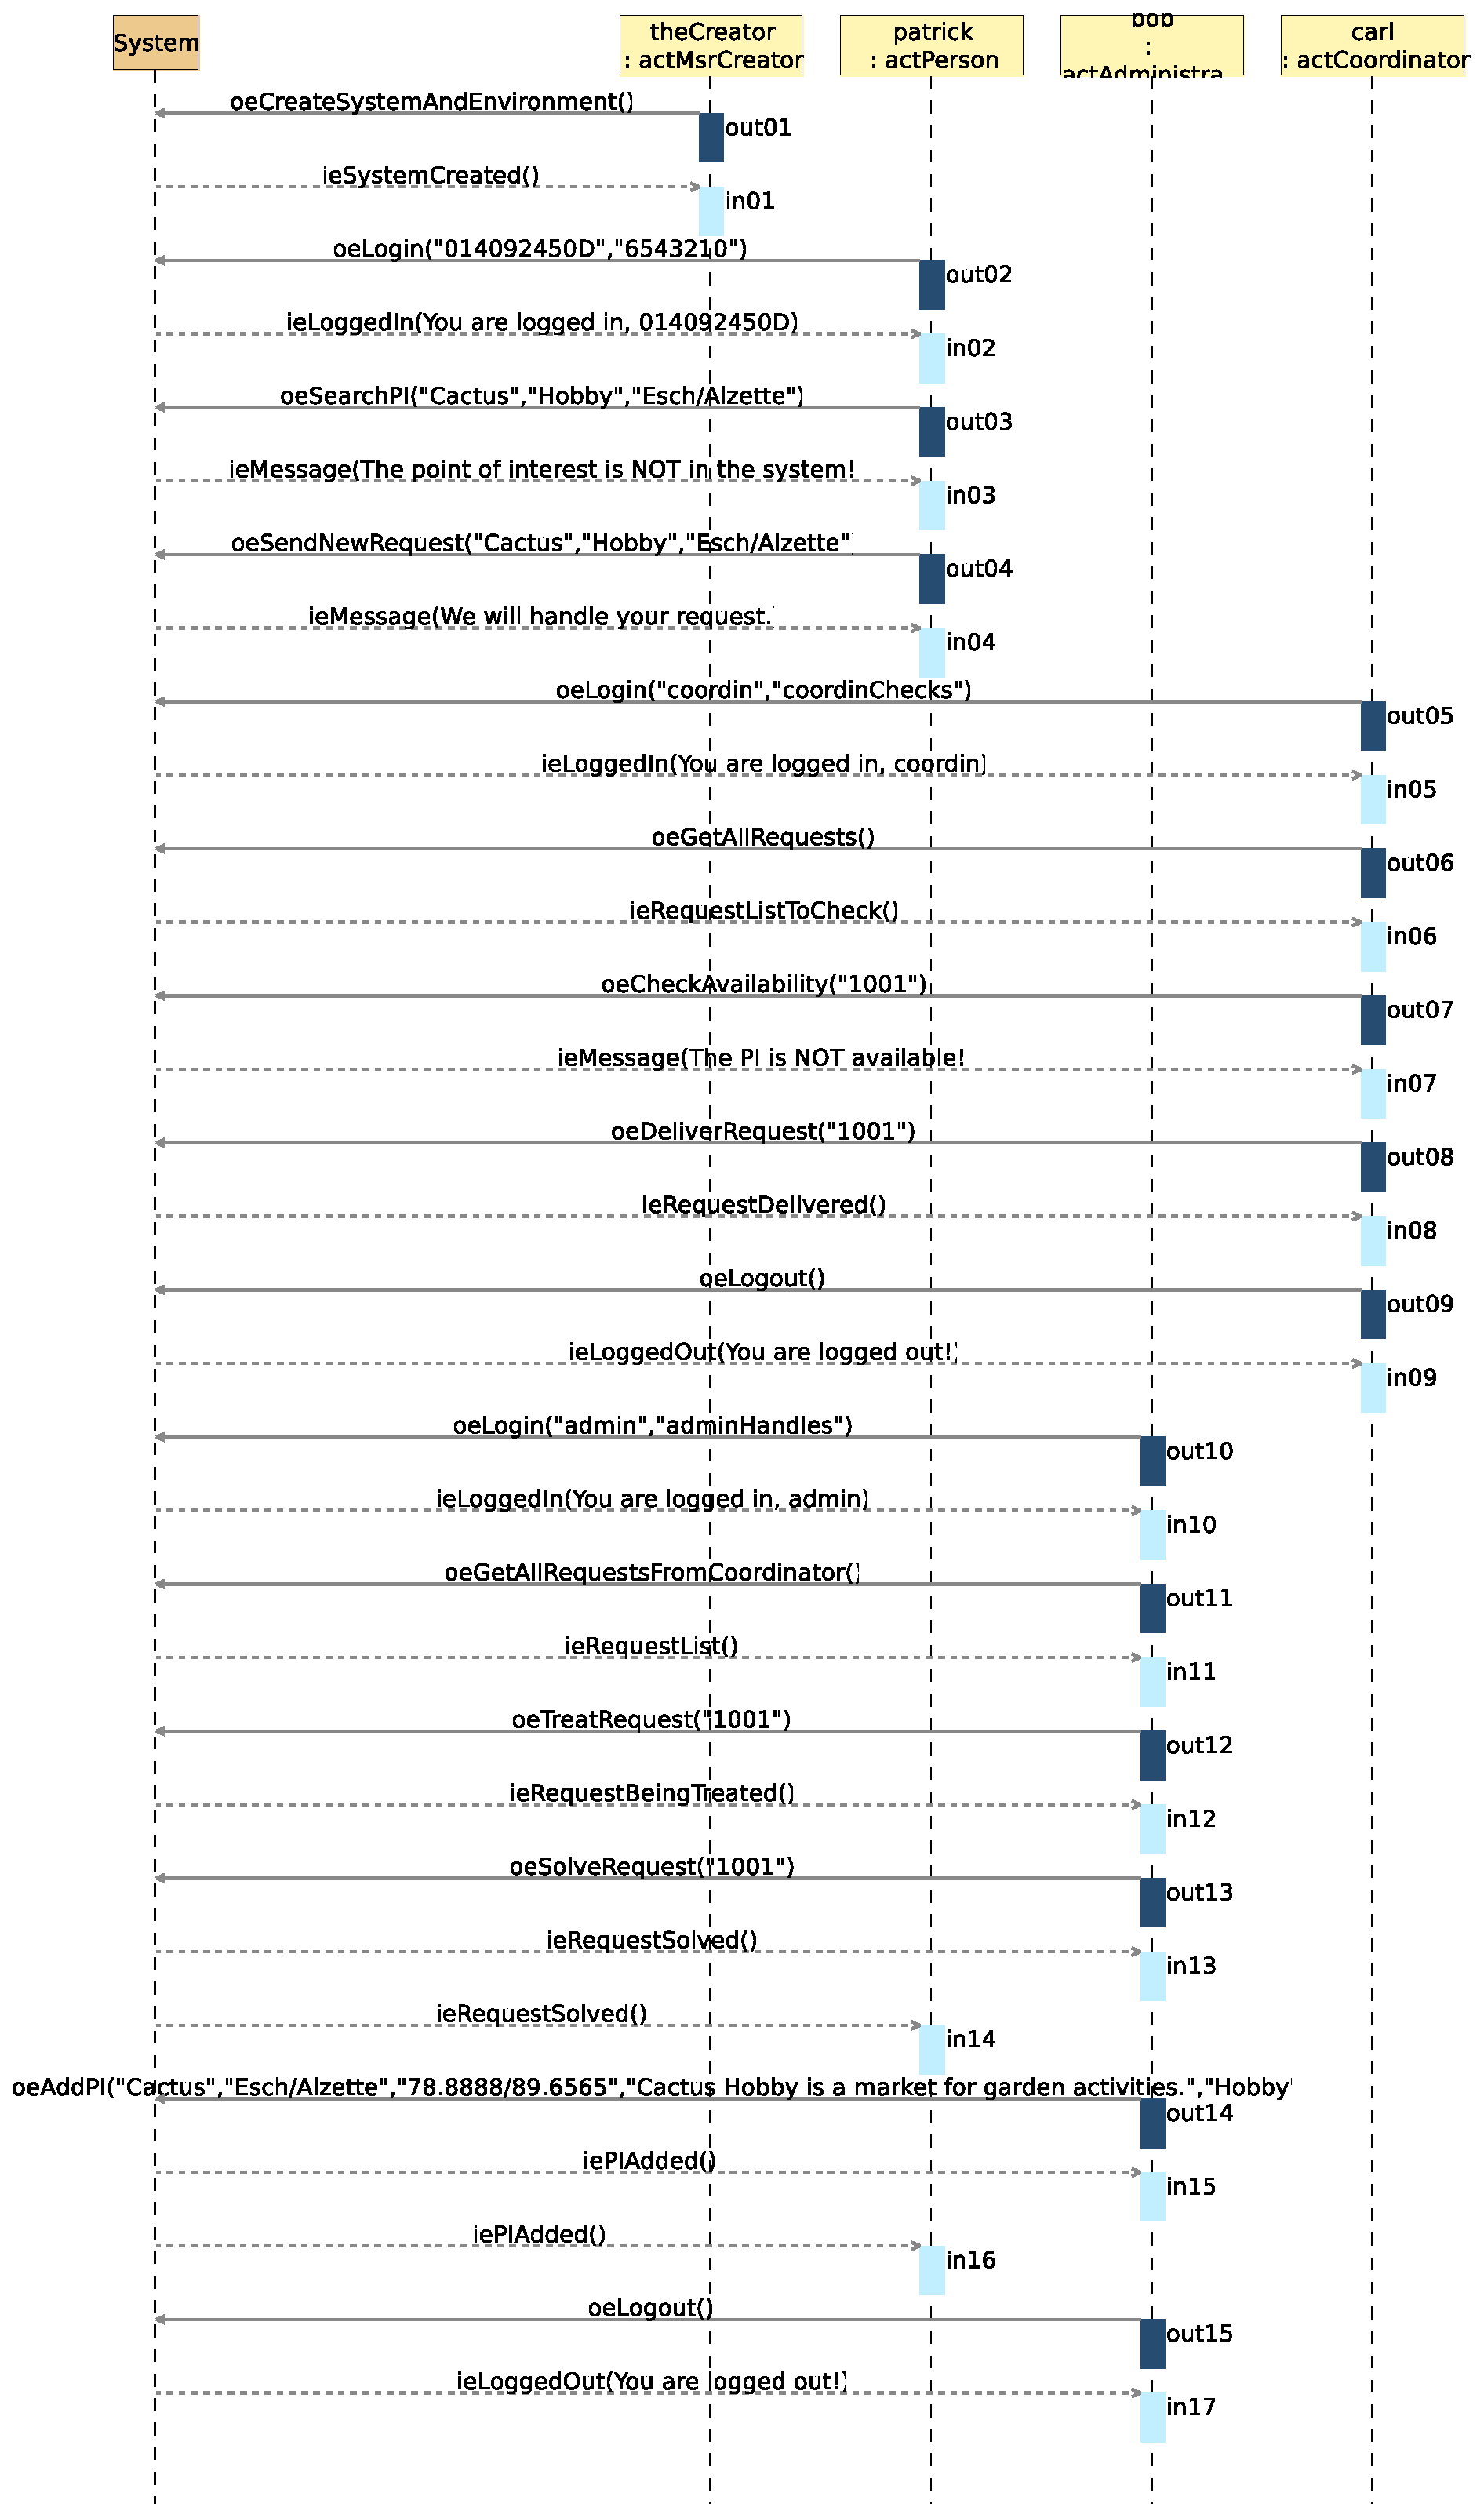
\includegraphics[
	angle=0
	]{./images-report-gen/usecase-model/summary/uci-ucisuAddNewPI.eps}
	\end{center}
	\caption[lu.uni.lassy.excalibur.MyCrash.G02 Sequence Diagram: uci-ucisuAddNewPI]{suAddNewPI summary use case instance}
	\label{fig:lu.uni.lassy.excalibur.MyCrash.G02-RE-UC-uci-ucisuAddNewPI}
	\end{figure}
	\vspace{0.5cm}
